\section{Security Considerations}
\label{sec:security}

In this last section we will take a look at some security considerations surrounding Roslyn. It is important to realize that the code base by itself is very hard to secure: there are several algorithms in it that have exponential or polynomial time -- executing a DoS\footnote{DoS: Denial of Service by flooding the application with work} is trivial since all you have to do is pass in the appropriate data. For this reason it is very hard to secure a compiler server\parencite{Gocke2015} since legitimate input and malicious input are virtually impossible to distinguish. However, there are some areas where we can identify a (shared) responsibility for developers in the way they utilize the Roslyn platform.

\subsection{Deterministic builds}
\label{sec:deterministic-builds}

\epigraph{With the number of dependencies present in large software projects, there is no way any amount of global surveillance, network censorship, machine isolation, or firewalling can sufficiently protect the software development process of widely deployed software projects in order to prevent scenarios where malware sneaks into a development dependency through an exploit in combination with code injection, and makes its way into the build process of software that is critical to the function of the world economy.}
{\textit{Mike Perry \\ \footnotesize{Deterministic Builds Part One: Cyberwar and Global Compromise\protect\footnotemark}}}

\footnotetext{\url{https://blog.torproject.org/blog/deterministic-builds-part-one-cyberwar-and-global-compromise}}

When it comes to security, one of the main guarantees you're interested is that the the file you have locally is the same as what has been audited by the vendor and/or community. A popular way to do this is by having the vendor/community create a hash of the application and store it publicly. Afterwards the user can download the binaries or source files (which can be anything from a small plugin to a full-fledged application), generate a hash from those files using the same algorithm and compare the results. Ideally, these two hashcodes should be the same. If they are not the same, there are three possible causes:

\begin{itemize}
\item The remote hash is outdated
\item The source files have been replaced (maliciously)
\item The application is not deterministic
\end{itemize}

In this section we will talk about the third option. It should be noted that at the time of writing deterministic builds have not been entirely implemented yet in the Roslyn code base but if the tracking issue \#372\footnote{\url{https://github.com/dotnet/roslyn/issues/372}} is any indication, there is only a limited amount of work left to be done.

\subsubsection{What makes a build deterministic?}
\label{sec:deterministic-builds-what}

\begin{displayquote}
"deterministic builds" -- packages which are byte-for-byte identical no matter who actually builds them, or what hardware they use.\parencite{Perry2013} 
\end{displayquote}

\noindent This definition immediately highlights the key idea behind deterministic builds: when a developer builds the Roslyn solution on his local machine, he should receive an identical result as if it had happened on Microsoft's build-servers. This is a harder task than it looks: it means that your code base can't contain any non-deterministic behaviour. While this might seem like an obvious conclusion, it implies that every single aspect of the code base that has an effect on its output must be implicitly or explicitly the same every time the code is built. 

As an example we can look at Roslyn issue \#223\footnote{\url{https://github.com/dotnet/roslyn/issues/223}} which specifies that in a certain scenario, anonymous types are emitted in a different order than expected. Looking closer at the diagnosis presented by the team we can see that the culprit seems to be the enumerating of dictionary entries.

Looking at the exact fix in PR \#948\footnote{\url{https://github.com/dotnet/roslyn/pull/948/files}} we see that the change consisted switching from a non-deterministic iteration to a deterministic one. When you iterate the \texttt{Values} property of a \texttt{Dictionary<K, V>} you do so in an unspecified order as we can read from the documentation:

\begin{displayquote}
The order of the values in the \texttt{Dictionary<TKey, TValue>.ValueCollection} is unspecified, but it is the same order as the associated keys in the \texttt{Dictionary<TKey, TValue>.KeyCollection} returned by the \texttt{Keys} property.\footnote{\url{https://msdn.microsoft.com/en-us/library/ekcfxy3x.aspx}}
\end{displayquote}

\noindent Indeed, the result was to switch from an undeterministic iteration (listing \ref{lst:undeterministic-values}) to a deterministic one by ordering the collection first (listing \ref{lst:deterministic-values}).

\lstset{style=csharp, caption={Undeterministic iteration of values}}
\begin{lstlisting}[label={lst:undeterministic-values}]
foreach (var template in anonymousTypes.Values)
\end{lstlisting}

\lstset{style=csharp, caption={Deterministic iteration of values}}
\begin{lstlisting}[label={lst:deterministic-values}]
foreach (var template in from kv in anonymousTypes 
												 orderby kv.Key 
												 select kv.Value)
\end{lstlisting}

\subsubsection{Other benefits to deterministic builds}
\label{sec:deterministic-builds-benefits}

The security aspect is a major reason to provide this characteristic to your code base but there are others:

\begin{itemize}
\item Reduces surprises by not relying on unspecified behaviour
\item Reduces I/O load by being able to skip a specific binary in certain situations if a binary with that exact hash is already stored\footnote{\label{ft:chromium}\url{https://www.chromium.org/developers/testing/isolated-testing/deterministic-builds}}
\item Reduces test execution time through the ability of re-using cached test results if the tested binary has not changed\textsuperscript{\ref{ft:chromium}}
\end{itemize}
\subsection{External analyzers}
\label{sec:security-external-analyzers}

Perhaps the most important security risk at all is the fact that the developer is adding external code to his development environment. There are no restrictions to what an analyzer can do: it could upload your source code to a remote server, it could search through your file system, it could download malware\footnote{Malware: malicious software} and hide it on your system, etc. This is not an uncommon risk however: people install extensions in their software all the time and Visual Studio is no exception to that: think about browser extensions or npm packages\footnote{npm: Node Package Manager -- Javascript-based scripts for the NodeJS platform} for example. 

An interesting attack vector here is that it's not something we're always aware of. For example you could be browsing a repository on Github when you suddenly decide to contribute so you fork the project and make alterations locally. What you didn't know, however, was that the project contained an analyzer which looked through your personal files, found a folder called 'my\_company\_repositories' and uploaded your proprietary code to locations unknown. At no point were you aware this was happening because analyzers are somewhat hidden in the sense that they're considered references (figure \ref{img:security-analyzers-solution-explorer}) but contrary to 'traditional' references, these are executed when the application isn't: as soon as you open a solution with a malicious analyzer, it has complete access to your system.

\begin{figure}[H]
\centering
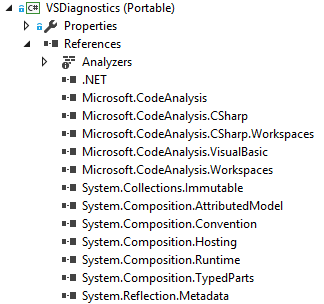
\includegraphics[scale=1]{security-analyzers-solution-explorer}
\caption[Analyzers amongst the project dependencies]{Analyzers amongst the project dependencies}
\label{img:security-analyzers-solution-explorer}
\end{figure}

That being said, in the end this is the same risk as with every other piece of software you download. Caution is advised anytime you download something from the internet and it's important to be aware of where things might be hidden.